\section{Answer-Conditioned Rationale (ACR) Filtering}
\label{app:filtering}

\subsection{ACR Generation}
\label{subsec:acr-generation}

For hard prompts, MinervaRL generates answer-conditioned rationale (ACR) traces by augmenting the original training prompt with a label-revealing block. The ACR prompt provides the ground-truth label(s), optionally includes a truncated canonical reference, and asks the model to produce a short justification that ends in the same final-answer format required by the original task. The prompt explicitly discourages leakage language, such as stating that the answer was provided. \Cref{fig:acr-template} shows the template.

\begin{figure}[t]
\centering
\begin{tcolorbox}[title=ACR Generation Prompt]
You are generating a reasoning trace for training.\\
\\
GROUND\_TRUTH\_LABELS:\\
- \textless LABEL\_1\textgreater\\
- \textless LABEL\_2\textgreater\\
\\
LABEL\_REFERENCE:\\
\textless details\_text\textgreater\\
\\
Instructions:\\
- Write a short reasoning that would justify selecting the correct label(s) from the input.\\
- \textless TASK\_OR\_ENTITY\_REASONING\_HINT\textgreater\\
- Do NOT say or imply that the answer was provided (no phrases like ``given the answer'', ``based on the provided label'', ``ground truth'', etc.).\\
- End with the final answer in the same format required by the original task.
\end{tcolorbox}
\caption{Answer-conditioned rationale (ACR) prompt template used to elicit training traces.}
\label{fig:acr-template}
\end{figure}

\subsection{Candidate Filtering and Selection}
\label{subsec:acr-filtering}

For each buffered training prompt with unique identifier (UID) $i$, ACR generation produces $K$ candidate traces $\{c_{i,k}\}_{k=1}^{K}$. MinervaRL retains at most one trace per UID for self-distillation. Filtering proceeds in three stages. First, each candidate is scored by the task-specific Minerva verifier, yielding a correctness score $s_{i,k}\in[0,1]$; only candidates with $s_{i,k}=1$ are considered for distillation. Second, verifier-correct candidates pass through heuristic filters that remove leakage and low-quality generations. Third, the remaining candidates are scored by a lightweight TextCNN quality classifier, and the highest-scoring eligible trace is selected.

\paragraph{Heuristic filters.}
We apply four heuristic checks before the ML filter. The leakage filter rejects candidates containing curated phrases or regex patterns that directly refer to provided labels, references, or ground-truth answers. The reasoning-length filter rejects candidates whose reasoning portion, excluding the final answer line, contains fewer than 100 characters. The grounding filter rejects candidates whose reasoning has Jaccard overlap below $0.05$ with the task description plus label reference, computed over lowercased alphanumeric tokens after removing ID-like tokens. Finally, the degeneracy filter rejects repetitive responses when the response has at least 30 tokens. Degeneracy checks include $n$-gram repetition thresholds, repeated-window checks, and near-duplicate sentence checks. Specifically, we reject if $\mathrm{rep}_3\ge 0.70$ or $\mathrm{rep}_4\ge 0.75$; if repeated windows of size 24 and stride 12 are exact matches or have 3-gram Jaccard similarity at least $0.9$; or if sentences within a 6-sentence window have SequenceMatcher similarity at least $0.75$ when both sentences contain at least 6 words. These thresholds apply only to the heuristic repetition checks; the TextCNN acceptance threshold is $\tau_q=0.5$.

\paragraph{TextCNN quality filter.}
Candidates that pass the heuristic filters are scored by the deployed response-only TextCNN classifier. The classifier tokenizes alphanumeric response tokens, truncates to at most 1024 tokens, and outputs a \textsc{good} probability $q_{i,k}\in[0,1]$. We keep candidates with $q_{i,k}\ge \tau_q$, where $\tau_q=0.5$. Let $L_{i,k}$ and $D_{i,k}$ denote whether candidate $k$ is rejected by leakage/quality heuristics or degeneracy heuristics, respectively. The eligible set is
\[
\mathcal{E}_i
=
\left\{
k
\;\middle|\;
s_{i,k}=1,\;
L_{i,k}=0,\;
D_{i,k}=0,\;
q_{i,k}\ge \tau_q
\right\}.
\]
If $\mathcal{E}_i=\varnothing$, UID $i$ contributes no distillation example in that interval. Otherwise, we select the highest-confidence candidate,
\[
k^\star
=
\arg\max_{k\in\mathcal{E}_i} q_{i,k},
\]
breaking ties uniformly at random. The selected distillation record pairs the original answer-free prompt with the accepted ACR response, i.e., $(x_i,c_{i,k^\star})$.

\subsection{Filtering Dynamics}
\label{subsec:filtering-dynamics}

\Cref{fig:filter-over-training} tracks the ACR filtering pipeline during training for Llama-3.1-8B-Instruct. We report the fraction of batches that pass the heuristic filter, pass the ML filter, and satisfy UID coverage, meaning that accepted traces span a sufficient number of distinct prompts. These rates increase over training, indicating that as the actor and EMA teacher improve, more ACR candidates are both verifier-correct and suitable for stable original-prompt distillation.

\begin{figure}[t]
  \centering
  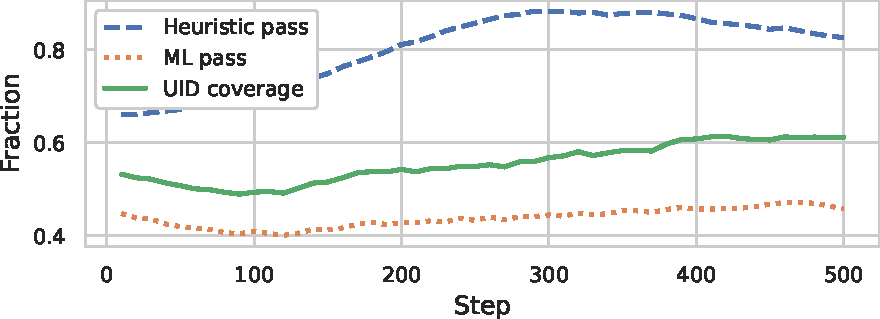
\includegraphics[width=0.8\linewidth]{figures/llama8b-acr-distill-fractions.pdf}
  \caption{Acceptance rates of the ACR self-distillation pipeline over training for Llama-3.1-8B-Instruct: fraction of batches passing the heuristic filter, passing the machine-learning (ML) filter, and meeting unique identifier (UID) coverage.}
  \label{fig:filter-over-training}
\end{figure}

\section{Training the TextCNN Reasoning-Quality Classifier}
\label{sec:textcnn-judge-training}

MinervaRL uses a lightweight TextCNN classifier to filter verifier-correct ACR traces before distillation. The classifier is trained to identify rationale quality rather than answer correctness: all training examples are already verifier-correct, and labels distinguish useful traces from traces with leakage, incoherence, unsupported reasoning, or other quality failures.

\subsection{Dataset Curation}
\label{subsec:textcnn-dataset-curation}

We construct the TextCNN training data from Minerva-CTI prompts. For each prompt, we generate responses in two formats: \emph{plain} responses from the original prompt, and \emph{hinted} responses from an ACR-style prompt containing the ground-truth label, a label reference, and an explicit training-trace marker. Responses are generated with a diverse set of open or open-weight instruction-tuned LLMs using typical decoding settings of temperature $0.7$ and maximum length 1024 new tokens.

To ensure that the classifier learns rationale quality rather than answer correctness, we first score all responses with the task verifier and retain only reward-correct responses with $\texttt{reward}=1$. These responses are then labeled \texttt{GOOD} or \texttt{BAD} by a rubric-based LLM judge. The judge does not re-grade correctness; instead, it marks a response as \texttt{BAD} if it exhibits any quality failure, including leakage, incoherence, unsupported claims, mismatch between rationale and final answer, answer-only reasoning, refusals, prompt copying, or other artifacts. The judge is instructed to return a single JSON object, as shown in \Cref{fig:llm-judge-prompt}.

\begin{figure}[t]
\centering
\begin{tcolorbox}[title=LLM Judge Prompt]
You are an expert CTI evaluator. You will be given a Question and a Response.\\
The Question may include answer/reference text as hints.\\[2pt]
Label the Response as GOOD or BAD. Mark BAD if any single criterion below is present;\\
otherwise mark GOOD. Do not grade correctness beyond these checks.\\[4pt]
Return exactly one JSON object on a single line and nothing else.\\
- GOOD: \{"label": "GOOD"\}\\
- BAD: \{"label": "BAD", "category\_id": \textless number\textgreater, "category\_title": "\textless title\textgreater"\}\\[4pt]
If multiple BAD criteria apply, choose the lowest-numbered category.\\[4pt]
Criteria (one per bullet):\\
1. Leakage: says or implies the answer/label/options/reference were provided,\\
\phantom{1. }or quotes/paraphrases provided reference text instead of reasoning from the prompt.\\
2. Incoherent: loops, repeated phrases/lines, templated filler, or gibberish.\\
3. Ungrounded: invents concrete details not in the question (extra CVEs,\\
\phantom{3. }vendors, malware names, IOCs, dates, techniques, etc.).\\
4. Mismatch: reasoning supports a different label than the final answer,\\
\phantom{4. }or directly contradicts it.\\
5. Unsupported: provides reasoning but does not use evidence from the prompt to\\
\phantom{5. }justify the answer (hand-wavy or irrelevant justification), OR provides an\\
\phantom{5. }answer with no reasoning at all (answer-only).\\
6. Other: refusals, policy/meta artifacts, generic CTI tutorials, or prompt copying.\\[6pt]
Example outputs:\\
\{"label": "GOOD"\}\\
\{"label": "BAD", "category\_id": 1, "category\_title": "Leakage"\}\\[6pt]
QUESTION:\\
\{QUESTION\}\\[4pt]
RESPONSE:\\
\{RESPONSE\}
\end{tcolorbox}
\caption{Prompt template used to label reward-correct responses as \texttt{GOOD}/\texttt{BAD} for training the TextCNN rationale-quality classifier.}
\label{fig:llm-judge-prompt}
\end{figure}

To improve coverage of failure modes, we also synthesize additional \texttt{BAD} examples by conditioning a generator on randomly sampled rubric violations. These synthetic examples are retained only if they remain verifier-correct. We then build a balanced dataset by downsampling to 32k \texttt{GOOD} and 32k \texttt{BAD} examples, and split each class 80/20 into train and validation partitions.

\subsection{TextCNN Model and Training}
\label{subsec:textcnn-training}

The deployed classifier uses response text only; prompt text is not concatenated to the input. Responses are tokenized with the regex tokenizer \texttt{[A-Za-z0-9\_]+}, lowercased, and truncated to a maximum of 1024 tokens. The vocabulary is built from the training split with \texttt{max\_vocab}=100{,}000 and \texttt{min\_freq}=2, using \texttt{<pad>} and \texttt{<unk>} as special tokens.

The model is a standard TextCNN: an embedding layer followed by 1D convolutions with kernel widths 3, 4, and 5; ReLU activations; max-over-time pooling; feature concatenation; dropout; and a two-way linear classifier. We train with AdamW and cross-entropy loss for 5 epochs using batch size 128. Hyperparameters are selected by grid search over learning rate $\{3{\times}10^{-4},6{\times}10^{-4},10^{-3},2{\times}10^{-3},4{\times}10^{-3}\}$, filters per kernel $\{256,384\}$, dropout $\{0,0.25\}$, embedding dimension $\{200,300\}$, and maximum response-token budget. The deployed model uses learning rate $6{\times}10^{-4}$, 384 filters per kernel, embedding dimension 300, dropout 0.25, maximum response length 1024 tokens, and threshold 0.5. On the balanced validation split, it achieves 0.826 accuracy and $F_1=0.828$.

\subsection{Validation and Error Analysis}
\label{subsec:textcnn-error-analysis}

\begin{table}[t]
\centering
\caption{Validation confusion matrix for the TextCNN reasoning-quality filter at threshold 0.5.}
\label{tab:textcnn-confusion}
\begin{tabular}{lrr}
\toprule
 & Predicted GOOD & Predicted BAD \\
\midrule
Actual GOOD & 5{,}375 & 1{,}025 \\
Actual BAD  & 1{,}206 & 5{,}194 \\
\bottomrule
\end{tabular}
\end{table}

\Cref{tab:textcnn-confusion} reports the validation confusion matrix. False positives are \texttt{BAD} responses accepted by the TextCNN. As shown in \Cref{tab:textcnn-fp-breakdown}, most false positives involve leakage: 738 of 1{,}206 false positives (61.2\%) explicitly or implicitly reveal access to the provided answer or reference. Other common false-positive categories are ungrounded claims (17.7\%) and rationale-answer mismatch (13.2\%). These errors are often fluent and plausible, which makes them difficult for a lightweight lexical classifier to reject.

A representative \texttt{scenario\_to\_attack\_technique} false positive received $p(\mathrm{GOOD})=0.829$ from TextCNN, but the judge labeled it \texttt{BAD}/Leakage because it implies access to the provided reference techniques:

\begin{tcolorbox}[breakable,colback=white,colframe=black!25,boxrule=0.4pt,arc=1pt,left=4pt,right=4pt,top=4pt,bottom=4pt]
\small
A malware has installed a bootkit on the system to maintain persistence.
A bootkit modifies the boot sectors of a hard drive, allowing malicious code to execute before the operating system has loaded.
This behavior aligns with the definition of techniques that involve modifying the operating system or firmware to achieve persistence.

The Master Boot Record (MBR) and Volume Boot Record (VBR) are key components involved in the boot process, and modifying these areas would allow an adversary to execute malicious code before the operating system loads.
This is a common method used by bootkits to persist on systems.

\emph{Considering the provided techniques}, the most suitable ID is \texttt{T1542.003}, which directly corresponds to Bootkit, as it describes the use of a bootkit to persist on systems.
Therefore, the selected technique ID is \texttt{T1542.003}.
\end{tcolorbox}

False negatives are \texttt{GOOD} responses rejected by the TextCNN. \Cref{tab:textcnn-fn-breakdown} shows that these are concentrated in open-ended ATT\&CK generation tasks, especially \texttt{scenario\_to\_attack\_mitigations} and \texttt{scenario\_to\_attack\_technique}. These tasks permit diverse valid rationales, so a compact response-only classifier can reject acceptable traces whose style differs from common \texttt{GOOD} examples. This error profile is consistent with the component ablations in \Cref{tab:eval12-ablation-summary}: removing the full filtering pipeline or only the ML filter reduces AthenaBench-Mini and average performance relative to full MinervaRL, despite occasional TextCNN errors.

\begin{table}[t]
\centering
\caption{False positives by LLM-judge rubric category for the TextCNN filter at threshold 0.5.}
\label{tab:textcnn-fp-breakdown}
\begin{tabular}{lrr}
\toprule
Rubric category & Count & Share of FP \\
\midrule
Leakage & 738 & 61.2\% \\
Ungrounded & 214 & 17.7\% \\
Mismatch & 159 & 13.2\% \\
Incoherent & 77 & 6.4\% \\
Unsupported & 18 & 1.5\% \\
\bottomrule
\end{tabular}
\end{table}

\begin{table}[t]
\centering
\caption{False negatives by task for the TextCNN filter at threshold 0.5.}
\label{tab:textcnn-fn-breakdown}
\small
\begin{tabular}{lrr}
\toprule
Task & Count & Share of FN \\
\midrule
\texttt{scenario\_to\_attack\_mitigations} & 392 & 38.2\% \\
\texttt{scenario\_to\_attack\_technique} & 194 & 18.9\% \\
\texttt{cve\_to\_cwe} & 173 & 16.9\% \\
\texttt{scenario\_to\_attack\_tactics} & 64 & 6.2\% \\
\texttt{sentinel\_to\_attack\_technique} & 35 & 3.4\% \\
\texttt{sigma\_to\_attack\_technique} & 35 & 3.4\% \\
\texttt{sigma\_to\_attack\_tactics} & 34 & 3.3\% \\
\texttt{cve\_to\_cvss\_v31} & 28 & 2.7\% \\
\texttt{threat\_actor} & 23 & 2.2\% \\
\texttt{art\_to\_attack\_technique} & 20 & 2.0\% \\
Other tasks & 27 & 2.6\% \\
\bottomrule
\end{tabular}
\end{table}
